\section{Results \& Discussion}

    In this section, I show some of our results and point out problems that occurred. The presented pictures are mostly of size 200X200.
    \subsection{Results after 7500 Epochs}\\
    After 7500 epochs, sometimes the outlines of houses are recognizable. Bright spots that might indicate a fire are partially set correctly. The brightness and intensity of the fire is relatively low. Example 1 and Example 2 can be interpreted as burning houses at night time.

    \begin{figure}[htb!] 
    	\centering
    	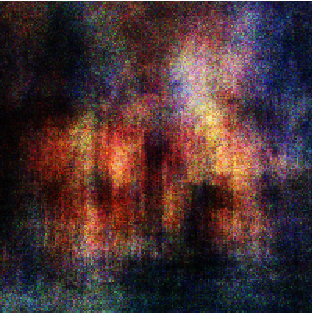
\includegraphics[width=0.7\linewidth]{7500-1.pdf}
    	\caption{Example 1: Door and Windows recognizable}
    	\label{fig:7500-1}
    \end{figure}
    
    %\pagebreak

    \begin{figure}[htb!] 
    	\centering
    	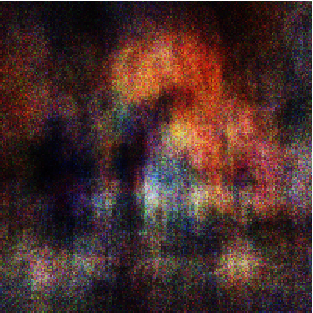
\includegraphics[width=0.7\linewidth]{7500-2.pdf}
    	\caption{Example 2: Double Pitch Roof}
    	\label{fig:7500-2}
    \end{figure}

    \begin{figure}[htb!] 
    	\centering
    	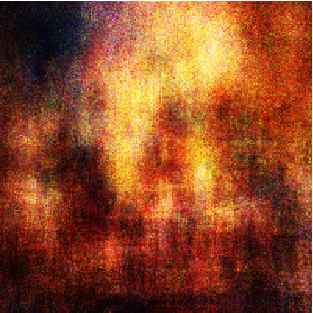
\includegraphics[width=0.7\linewidth]{7500-3.pdf}
    	\caption{Example 3: Mix of Example 1 and 2}
    	\label{fig:7500-3}
    \end{figure}
    
    \pagebreak
   
    \subsection{Results after 10000 Epochs}\\
        At around 10000 epochs, the fire reaches the desired intensity. The outlines that could be interpreted as houses are slowly disappearing.
    
    \begin{figure}[htb!] 
    	\centering
    	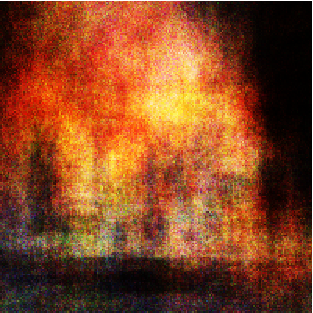
\includegraphics[width=0.7\linewidth]{10000-1.pdf}
    	\caption{Example 4: Fire in House Shape}
    	\label{fig:10000-1}
    \end{figure}

    \begin{figure}[htb!] 
    	\centering
    	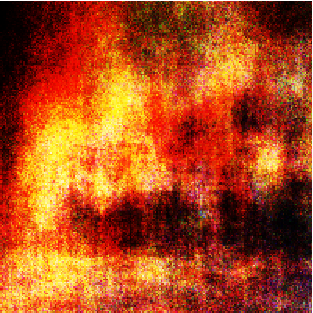
\includegraphics[width=0.7\linewidth]{10000-2.pdf}
    	\caption{Example 5: Windows discernable}
    	\label{fig:10000-2}
    \end{figure}

    \begin{figure}[htb!] 
    	\centering
    	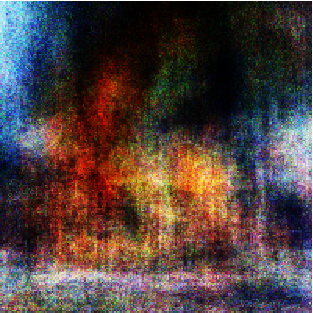
\includegraphics[width=0.7\linewidth]{10000-3.pdf}
    	\caption{Example 6: House with Smoke on Top}
    	\label{fig:10000-2}
    \end{figure}


    \subsection{Results after 15500 Epochs}\\    
    The picture becomes a mixture of yellow, red and black sections. It will overlap the point to see anything other than fire. The red tones might even be interpreted as lava.

    \begin{figure}[htb!] 
    	\centering
    	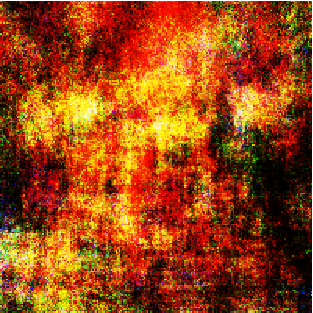
\includegraphics[width=0.7\linewidth]{15500-1.pdf}
    	\caption{Example 7}
    	\label{fig:15500-1}
    \end{figure}    

    \begin{figure}[htb!] 
    	\centering
    	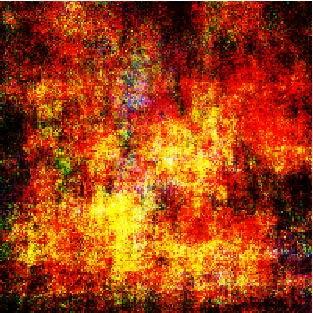
\includegraphics[width=0.7\linewidth]{15500-2.pdf}
    	\caption{Example 8}
    	\label{fig:15500-2}
    \end{figure} 

    \begin{figure}[htb!] 
    	\centering
    	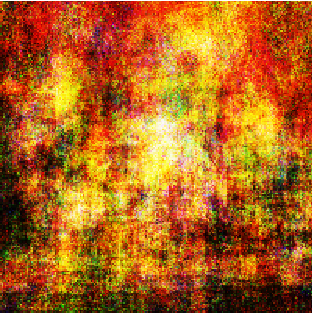
\includegraphics[width=0.7\linewidth]{15500-3.pdf}
    	\caption{Example 9}
    	\label{fig:15500-3}
    \end{figure} 

    \subsection{More Examples}\\
    Those pictures are of smaller size, 75X75 to be precise, after 10000 epochs. \\
    \begin{figure}[htb!]
    \centering
        \begin{subfigure}[htb!]{0.3\linewidth}
        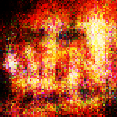
\includegraphics[width=\linewidth]{10000-1(7575).pdf}
        \caption{}
        \end{subfigure}
        \begin{subfigure}[htb!]{0.3\linewidth}
        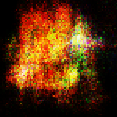
\includegraphics[width=\linewidth]{10000-2(7575).pdf}
        \caption{}
        \end{subfigure}
        \begin{subfigure}[htb!]{0.3\linewidth}
        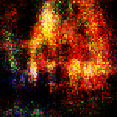
\includegraphics[width=\linewidth]{10000-3(7575).pdf}
        \caption{}
        \end{subfigure}
        \begin{subfigure}[htb!]{0.3\linewidth}
        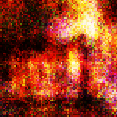
\includegraphics[width=\linewidth]{10000-4(7575).pdf}
        \caption{}
        \end{subfigure}
        \caption{Samples with 75X75 pixels.}
        \label{fig:coffee3}
    \end{figure}


\subsection{Problems}
\\
Unfortunately, fire is by far the most dominant feature in our dataset. In addition, the structure of the second important feature, the houses, is more difficult to recognize because it is composed of several more complex features. While in the case of fire, basically only the transition from yellow to red areas has to be learned, a house has significantly more criteria to go through as such. This includes vertical side walls, windows, in most cases tapered roofs, etc. In addition, resizing means that even more meaningfulness disappears because fine structures can no longer be perceived because they blur. This problem could be seen as a kind of mode collapse based initiated by the Discriminator. Mode collapse normally means that the Generator specializes itself mapping only one distribution, for example that of cats, since those images previously have been successfully accepted, even though dogs are also included in the data set. In our case the quality of the houses is not sufficient so that the Discriminator fails to incorporate this feature in his decision process whether to accept or reject the picture. Hence, the Generator fulfills its task by only producing images with fire since that it is all it takes to get the approval of the Discriminator. \\
